\documentclass[a4paper, 12pt]{article}

\usepackage{multirow}
\usepackage[table,xcdraw]{xcolor}
\usepackage{enumerate}
\usepackage{graphicx}
\usepackage[T5]{fontenc}
\usepackage[utf8]{inputenc}
\usepackage[margin = 2cm]{geometry}
\usepackage{amsfonts, amsmath, amssymb}
\usepackage[none]{hyphenat}
\usepackage{fancyhdr}
\usepackage{float}
\usepackage{hyperref}
\usepackage{caption}
\usepackage[nottoc, notlot, notlof]{tocbibind}

\captionsetup[table]{skip=5pt}
\pagestyle{fancy}
\fancyhead[L]{Trường Đại học Khoa học Tự nhiên - ĐHQG TP.HCM}
\fancyhead[R]{Nhóm Just $4^{th}$}

\begin{document}
\begin{titlepage}
    \begin{center}
        \vspace*{1cm}
        \Large\textbf{Trường Đại học Khoa học Tự nhiên\\Đại học Quốc gia TP.HCM}\\

        \vfill
        \line(1,0){450}\\[4mm]
        \LARGE\textbf{\MakeUppercase{Tiền xử lý dữ liệu}}\\[3mm]
        \Large{Khai thác dữ liệu \& Ứng dụng}\\[3mm]
        \Large{Nguyễn Bảo Long - MSSV: 18120201}\\
        \Large{Huỳnh Long Nam - MSSV: 18120212}
        \line(1,0){430}\\
        \vfill

        \vfill
        TP Hồ Chí Minh, ngày 20/10/2020
    \end{center}
\end{titlepage}

\tableofcontents
\thispagestyle{empty}
\clearpage

\section{Thông tin chung}

\begin{enumerate}
    \item Link GitHub: \url{https://github.com/baolongnguyenmac/DataMining-Lab1}
    \item Thông tin thành viên nhóm
    \begin{table}[H]
        \begin{center}
            \begin{tabular}{|c|c|c|c|}
            \hline
            STT & Họ tên          & MSSV     & Email                         \\ \hline
            1   & Nguyễn Bảo Long & 18120201 & 18120201@student.hcmus.edu.vn \\ \hline
            2   & Huỳnh Nam Long  & 18120212 & 18120212@student.hcmus.edu.vn         \\ \hline
            \end{tabular}
            \caption{Bảng thông tin thành viên nhóm}
        \end{center}
    \end{table}

    \item Tỷ lệ tham gia công việc
    \begin{table}[H]
        \begin{center}
            \begin{tabular}{|c|c|c|l|c|}
            \hline
            STT & MSSV     & \multicolumn{2}{c|}{Công việc}                & Tỷ lệ hoàn thành \\ \hline
            1 & \begin{tabular}[c]{@{}c@{}}18120201\\ 18120212\end{tabular} & Yêu cầu 1                  & Cài đặt Weka                     & 100\% \\ \hline
            2 & 18120212                                                    & \multirow{3}{*}{Yêu cầu 2} & Đọc dữ liệu vào Weka             & 100\% \\ \cline{1-2} \cline{4-5} 
            3   & 18120212 &  & Khám phá tập dữ liệu Weather               & 100\%            \\ \cline{1-2} \cline{4-5} 
            3   & 18120201 &  & Khám phá tập dữ liệu tín dụng Đức          & 100\%            \\ \hline
            4 & 18120201                                                    & \multirow{8}{*}{Yêu cầu 3} & Liệt kê các cột bị thiếu dữ liệu & 100\% \\ \cline{1-2} \cline{4-5} 
            5   & 18120201 &  & Đếm số dòng bị thiếu dữ liệu               & 100\%            \\ \cline{1-2} \cline{4-5} 
            6   & 18120201 &  & Điền giá trị bị thiếu                      & 100\%            \\ \cline{1-2} \cline{4-5} 
            7   & 18120201 &  & Xoá các dòng bị thiếu với ngưỡng cho trước & 100\%            \\ \cline{1-2} \cline{4-5} 
            8   & 18120201 &  & Xoá các cột bị thiếu với ngưỡng cho trước  & 100\%            \\ \cline{1-2} \cline{4-5} 
            9   & 18120212 &  & Xoá các mẫu bị trùng lặp                   & 100\%            \\ \cline{1-2} \cline{4-5} 
            10  & 18120212 &  & Chuẩn hoá một thuộc tính                   & 100\%            \\ \cline{1-2} \cline{4-5} 
            11  & 18120212 &  & Tính giá trị biểu thức                     & 100\%            \\ \hline
            12  & 18120201 & \multicolumn{2}{l|}{Viết }   & 100\%            \\ \hline
            13  & 18120201 & \multicolumn{2}{l|}{Trình bày báo cáo}        & 100\%            \\ \hline
            \end{tabular}
            \caption{Bảng phân chia công việc và mức độ hoàn thành}
        \end{center}
    \end{table}
\end{enumerate}

\clearpage

\section{Yêu cầu 1: Cài đặt Weka}
\subsection{Giao diện chức năng Explorer sau khi cài đặt Weka}
\begin{figure}[H]
    \begin{center}
        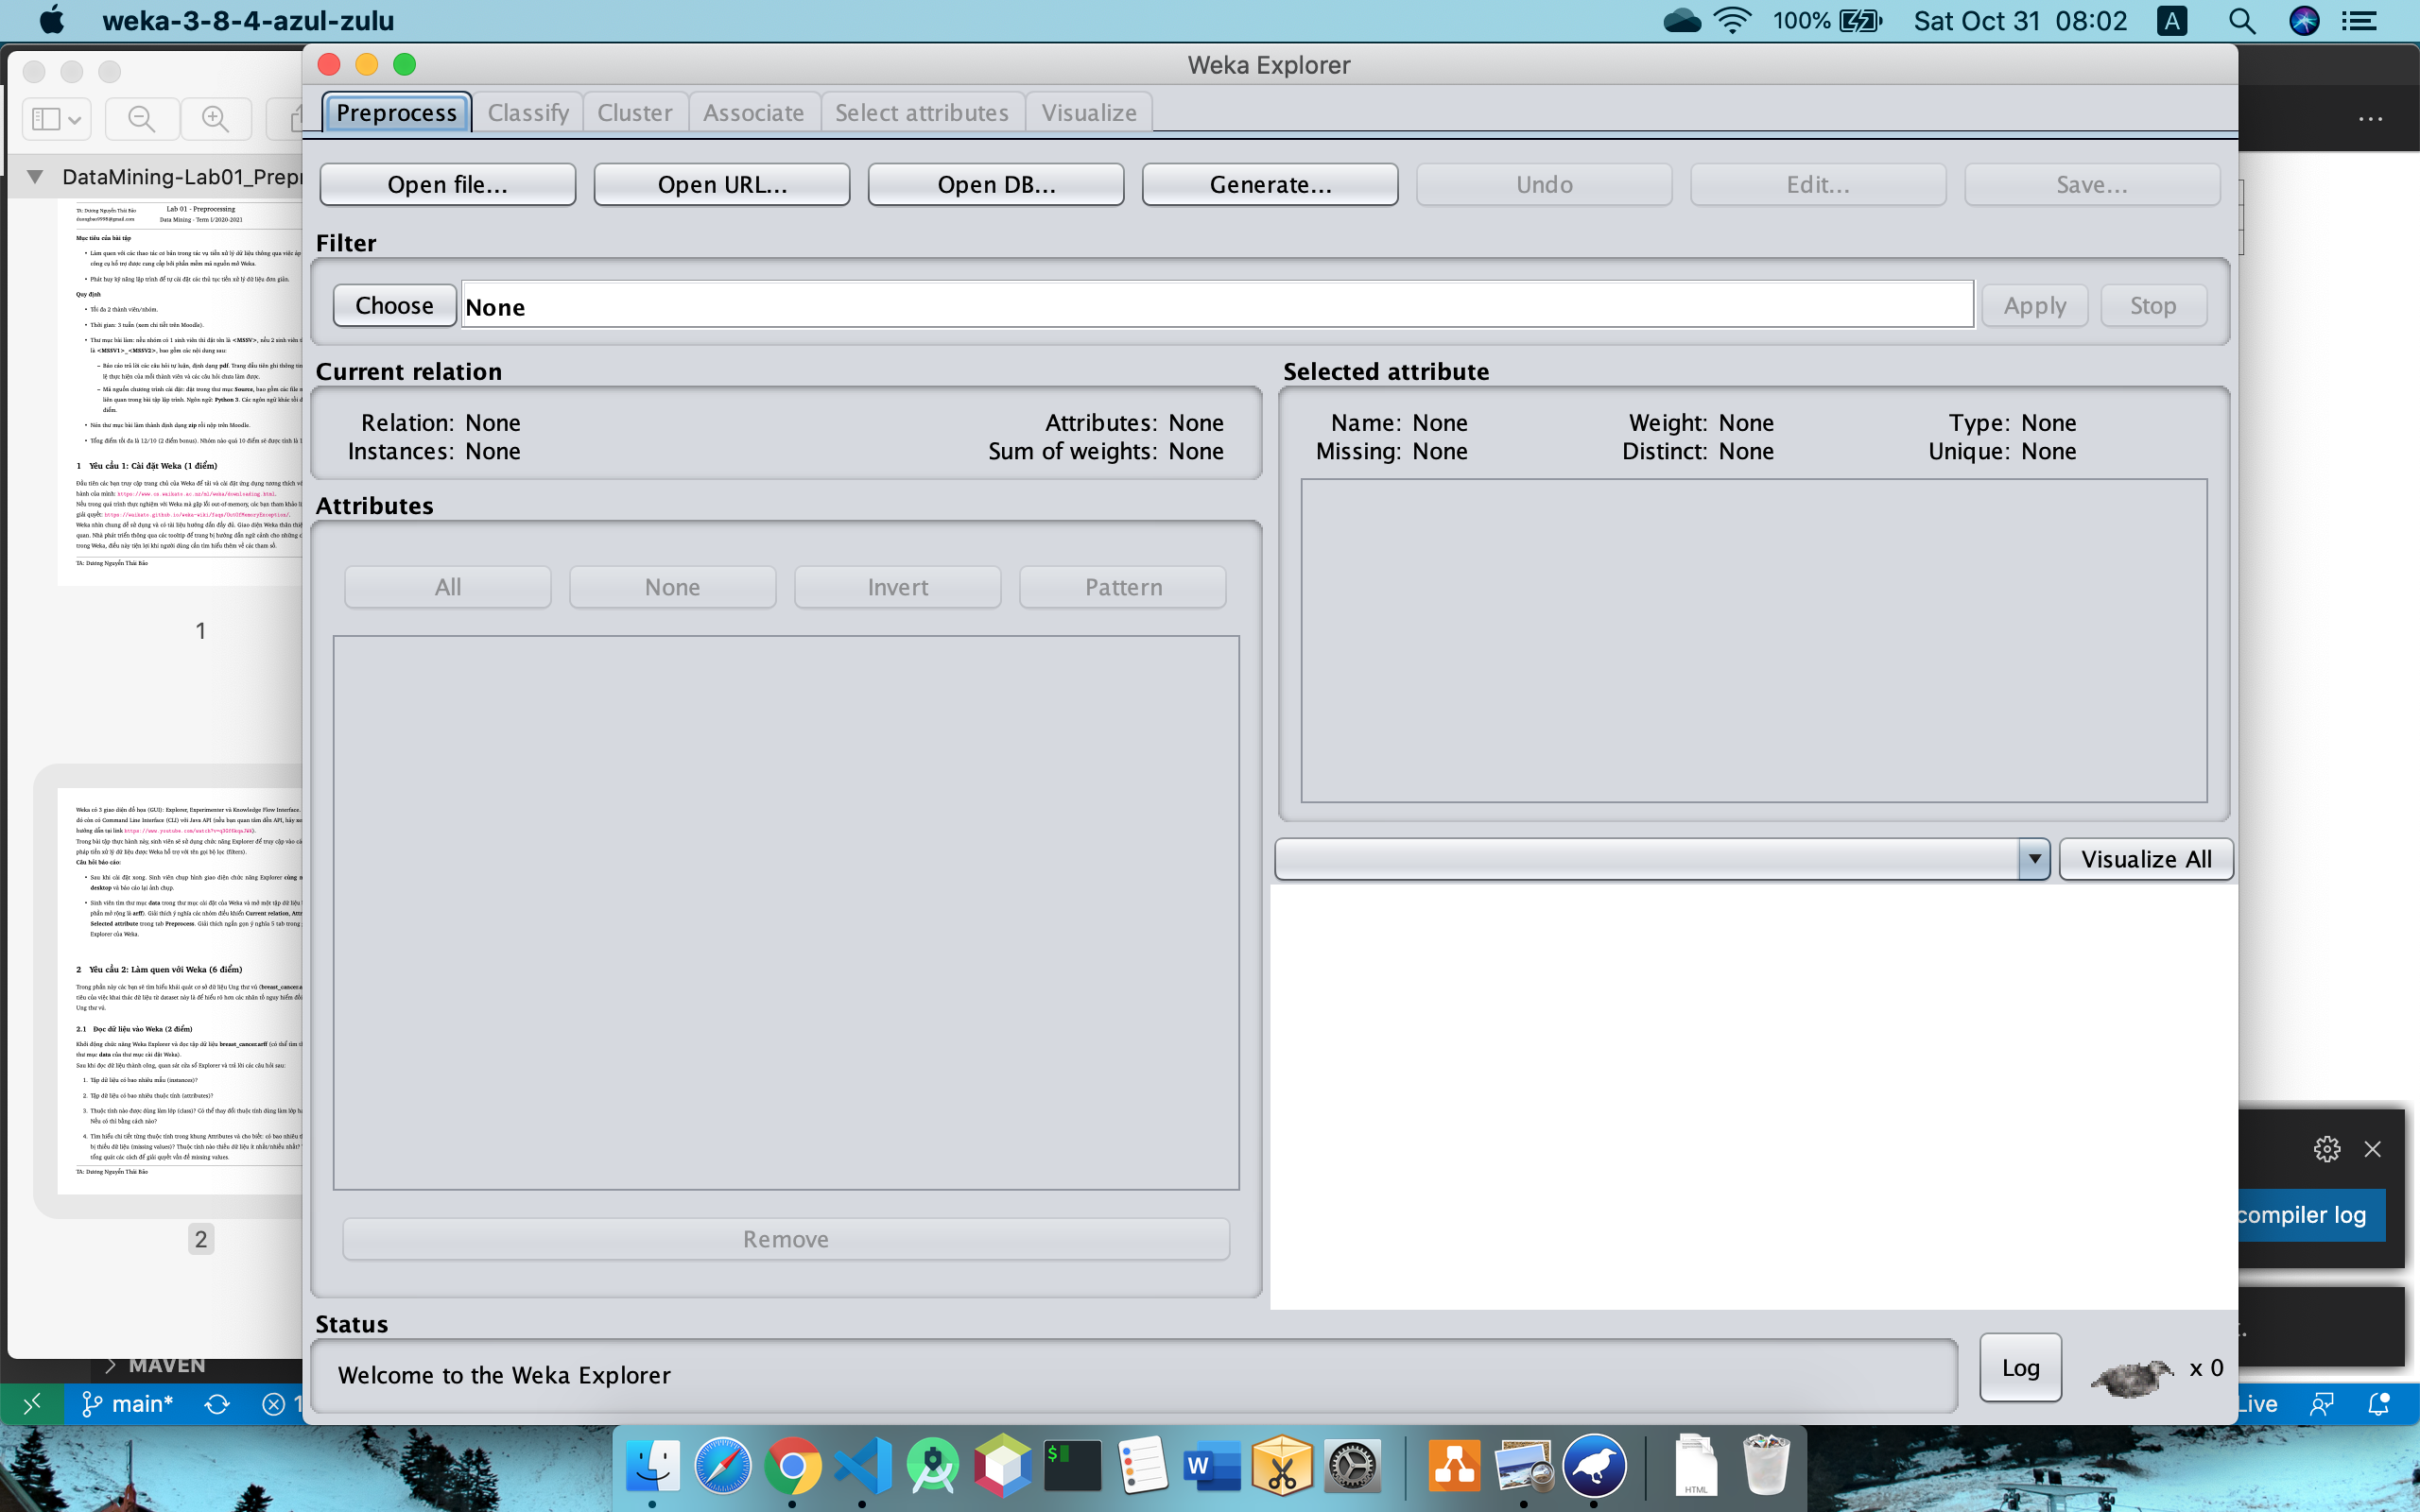
\includegraphics[scale = 0.35]{./images/wekw_explorer.png}
        \caption{Giao diện chức năng Explorer của Weka}
    \end{center}
\end{figure}

\subsection{Giải thích ý nghĩa các nhóm điều khiển và các tabs trên giao diện}
\begin{enumerate}
    \item Ý nghĩa nhóm lệnh điều khiển trong tab PreProcess
    \begin{itemize}
        \item Current relation (tạm dịch `Quan hệ hiện tại'): Cho biết các thông tin chung về tập dữ liệu hiện tại như tên tập dữ liệu, số mẫu, số thuộc tính
        \item Attributes (tạm dịch `Thuộc tính'): Cho biết danh sách các thuộc tính hiện tại trong tập dữ liệu
        \item Selected attribute (tạm dịch `Thuộc tính được chọn'): Cho biết thông tin chung liên quan đến thống kê (trong TH dữ liệu là dạng số) như trung bình cộng, giá trị min, giá trị max của thuộc tính đã được chọn trước trong phần \textbf{Attributes}. Đối với dữ liệu dạng định danh, Weka sẽ cung cấp danh sách các định danh và số lượng mỗi định danh
    \end{itemize}

    \item Ý nghĩa của các tabs
    \begin{itemize}
        \item PreProcess: Tiền xử lý dữ liệu (tab mặc định)
        \item Classify: Phân lớp dữ liệu
        \item Cluster: Gom cụm dữ liệu
        \item Associate: Khai phá các luật kết hợp
        \item Select Attributes: Lựa chọn thuộc tính. Sử dụng khi cần xem xét mối tương quan giữa các thuộc tính
        \item Visualize: Trực quan hoá dữ liệu
    \end{itemize}
\end{enumerate}

\section{Yêu cầu 2: Làm quen với Weka}

\subsection{Đọc dữ liệu vào Weka}

\begin{itemize}
    \item Mở tập dữ liệu \textbf{breast\_cancer.arff} trong giao diện Weka Explorer
    \item Explore dữ liệu
    \begin{itemize}
        \item Tập dữ liệu có 286 mẫu
        \item Tập dữ liệu có 10 thuộc tính
        \begin{figure}[H]
            \begin{center}
                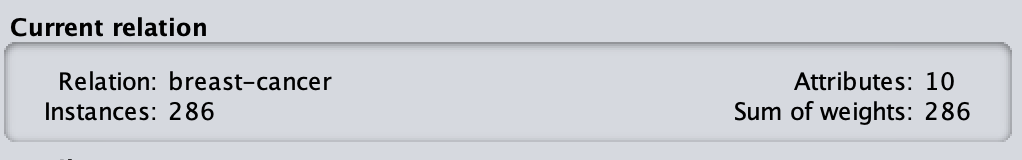
\includegraphics[scale = 0.75]{images/attribute_instance.png}
                \caption{Số lượng mẫu và thuộc tính của tập dữ liệu \textbf{breast\_cancer.arff}}
            \end{center}
        \end{figure}
        \item Thuộc tính "Class" là thuộc tính class của tập dữ liệu với 2 giá trị recurrence-events và no-recurrence-events được dùng làm lớp. Có thể thay đổi thuộc tính dùng làm lớp bằng cách chọn nút \textbf{Edit}, nhấp phải chuột tại thuộc tính mới và chọn \textbf{Attribute as class}
        \begin{figure}[H]
            \begin{center}
                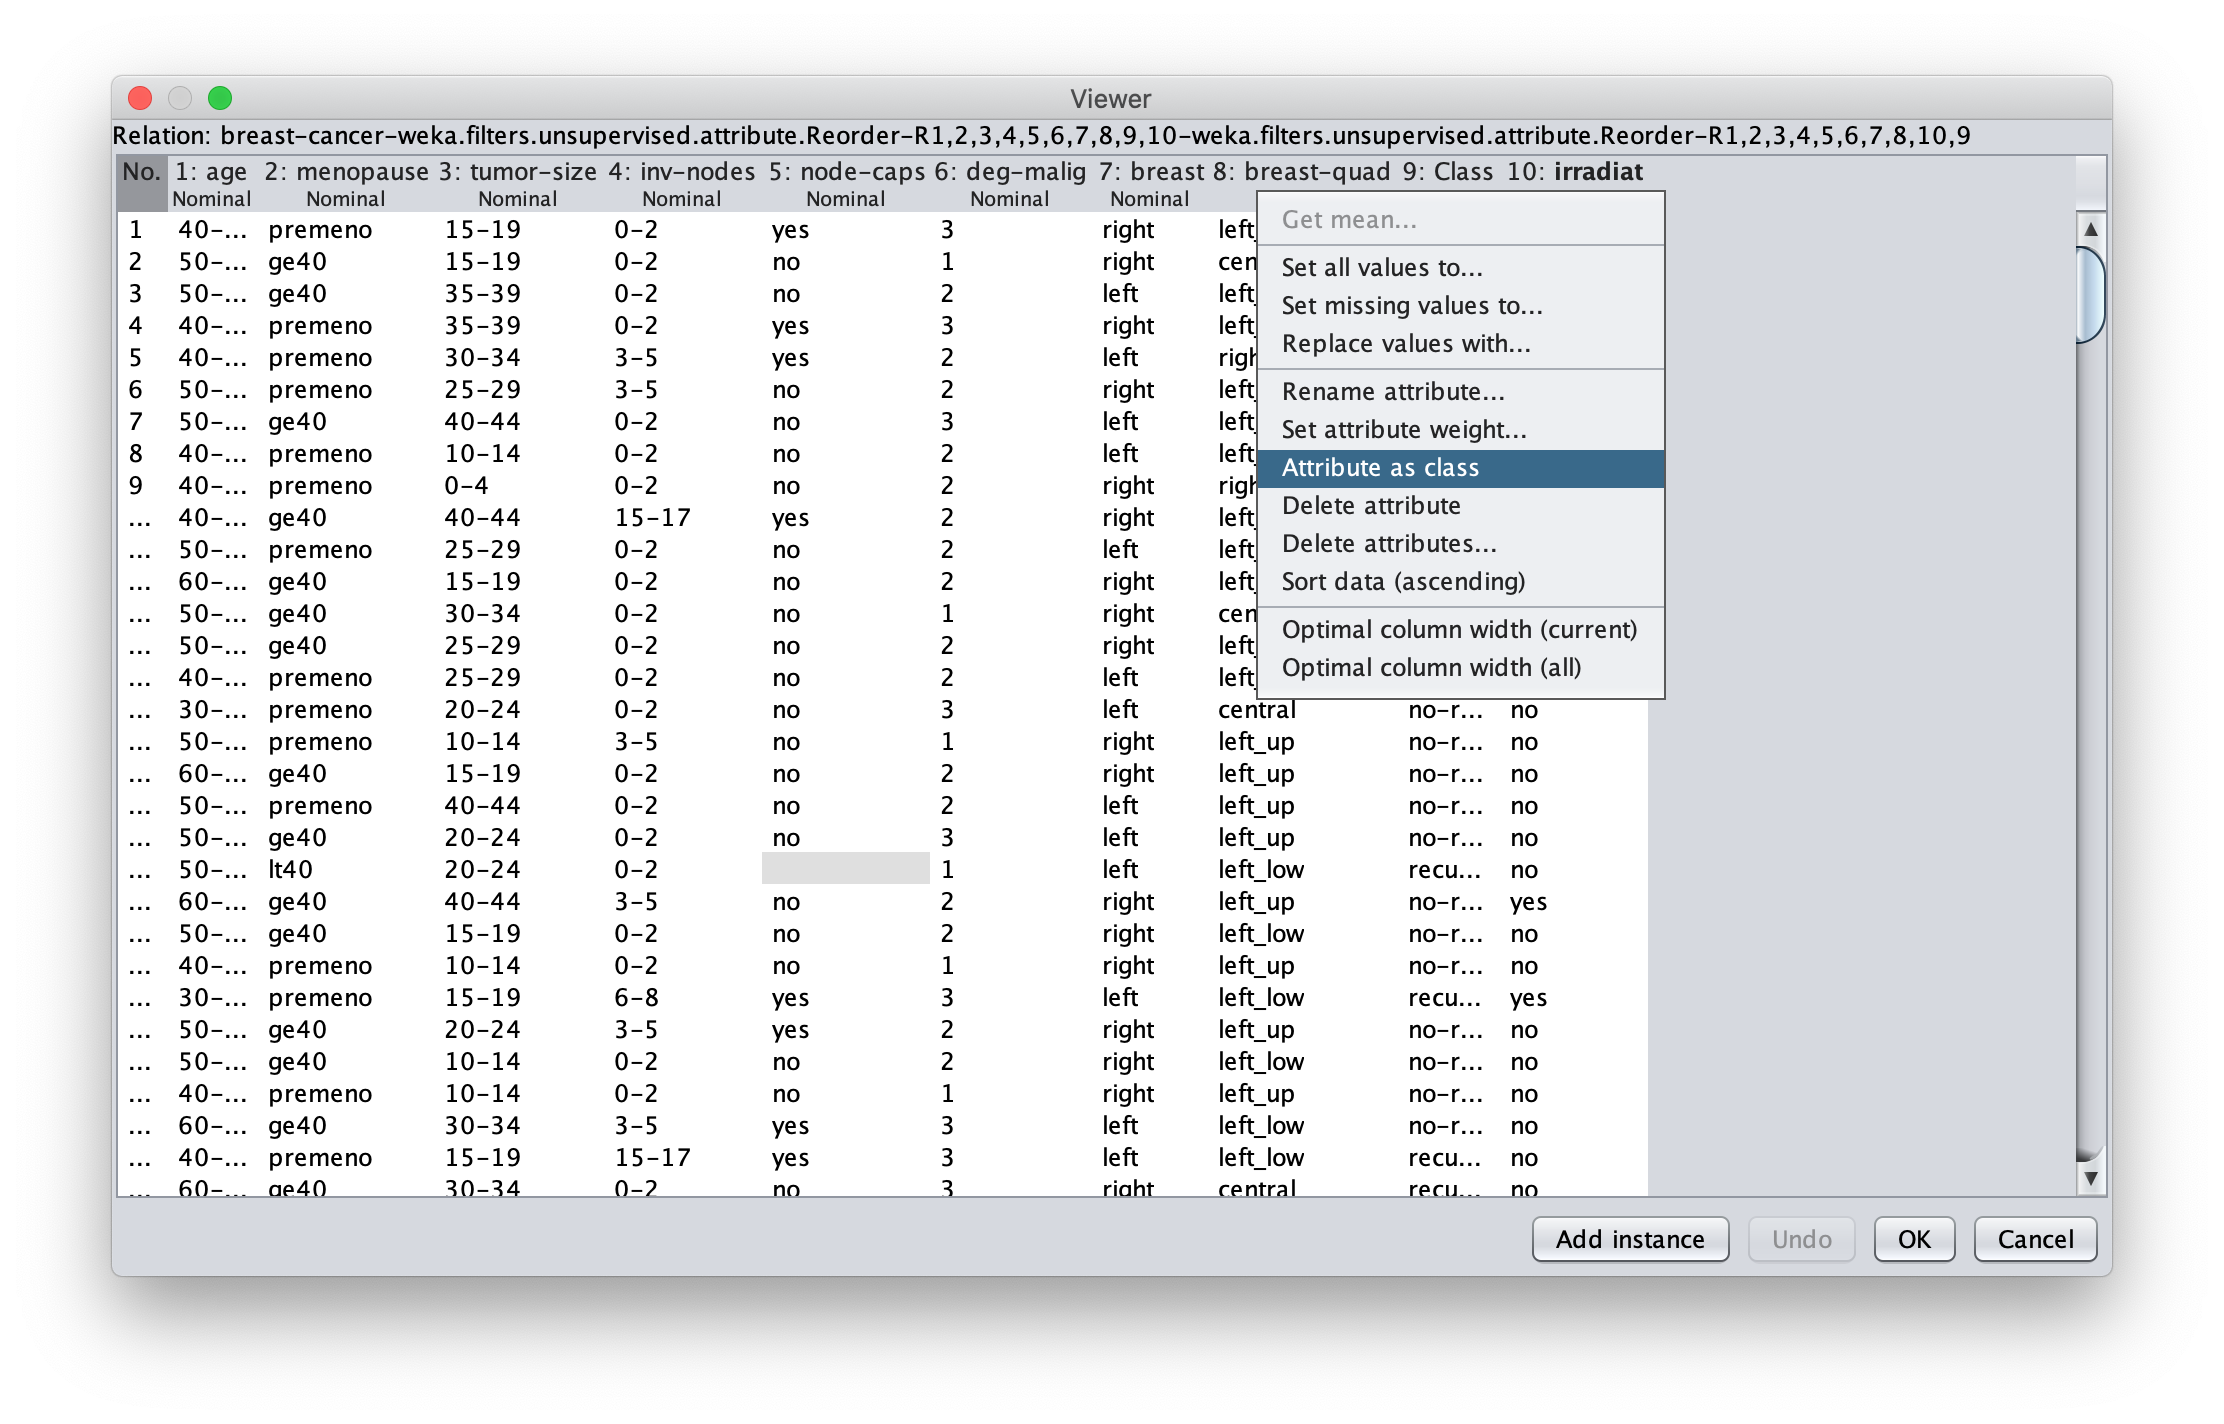
\includegraphics[scale = 0.45]{./images/changeClass.png}
                \caption{Thay đổi thuộc tính được dùng làm lớp}
            \end{center}
        \end{figure}

        \item Có 2 thuộc tính bị thiếu dữ liệu là \textbf{node\_caps} và \textbf{breast\_quad}. Trong đó, \textbf{node\_caps} thiếu nhiều nhất (thiếu 8 mẫu, tương đương 3\%) và \textbf{breast\_quad} thiếu ít nhất (thiếu 1 mẫu, tương đương gần 0\%)
        \begin{figure}[H]
            \begin{center}
                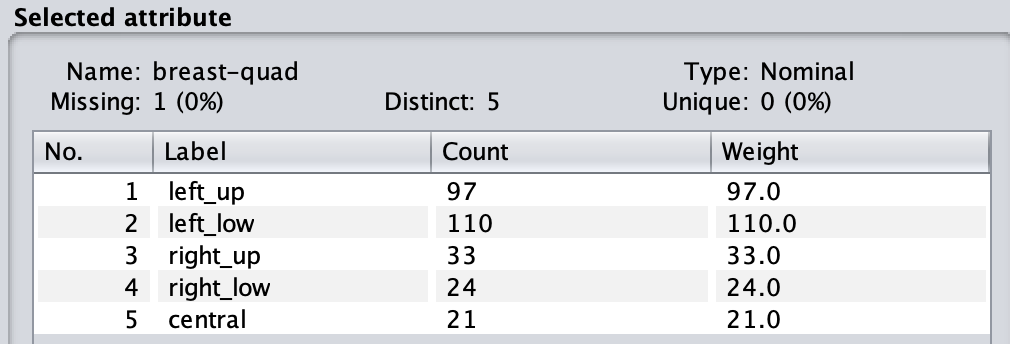
\includegraphics[scale = 0.65]{images/breast_quad_missingData.png}
                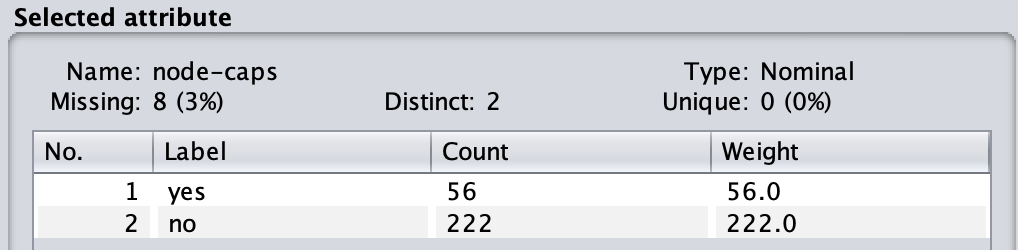
\includegraphics[scale = 0.65]{images/node_caps_missingData.png}
                \caption{Thuộc tính \textbf{node\_caps} và \textbf{breast\_quad} bị thiếu dữ liệu}
            \end{center}
        \end{figure}

        \item Khi gặp tình trạng thiếu dữ liệu, ta có thể loại bỏ dữ liệu thiếu đó hoặc bổ sung dữ liệu thiếu (bằng phương pháp lấy trung bình hoặc kNN)
        \item Có thể đặt tên cho đồ thị này là đồ thị phân bố lớp. Màu xanh biểu thị tại mỗi khoảng dữ liệu của attribute được chọn, có bao nhiêu mẫu cho kết quả no-recurrence-events. Tương tự với màu đỏ, cho kết quả recurrence-events
    \end{itemize}
\end{itemize}

\subsection{Khám phá tập dữ liệu Weather}

\begin{itemize}
    \item Tập dữ liệu có 5 thuộc tính và 14 mẫu
    \begin{itemize}
        \item Thuộc tính định danh: outlook, windy, play
        \item Thuộc tính số: temperature, humidity
    \end{itemize}

    \item Five-number summary của thuộc tính temperature và humidity
    \begin{table}[H]
        \begin{center}
            \begin{tabular}{|c|c|c|c|c|c|}
            \hline
                        & Min & Q1 & Mean   & Q3 & Max \\ \hline
            Temperature & 64  & 69 & 73.571 & 80 & 85  \\ \hline
            Humidity    & 65  & 70 & 81.643 & 90 & 96  \\ \hline
            \end{tabular}
            \caption{Bảng Five-number summary của thuộc tính temperature và humidity }
        \end{center}
    \end{table}

    \item Đồ thị biểu diễn các thuộc tính của tập dữ liệu
    \begin{figure}[H]
        \begin{center}
            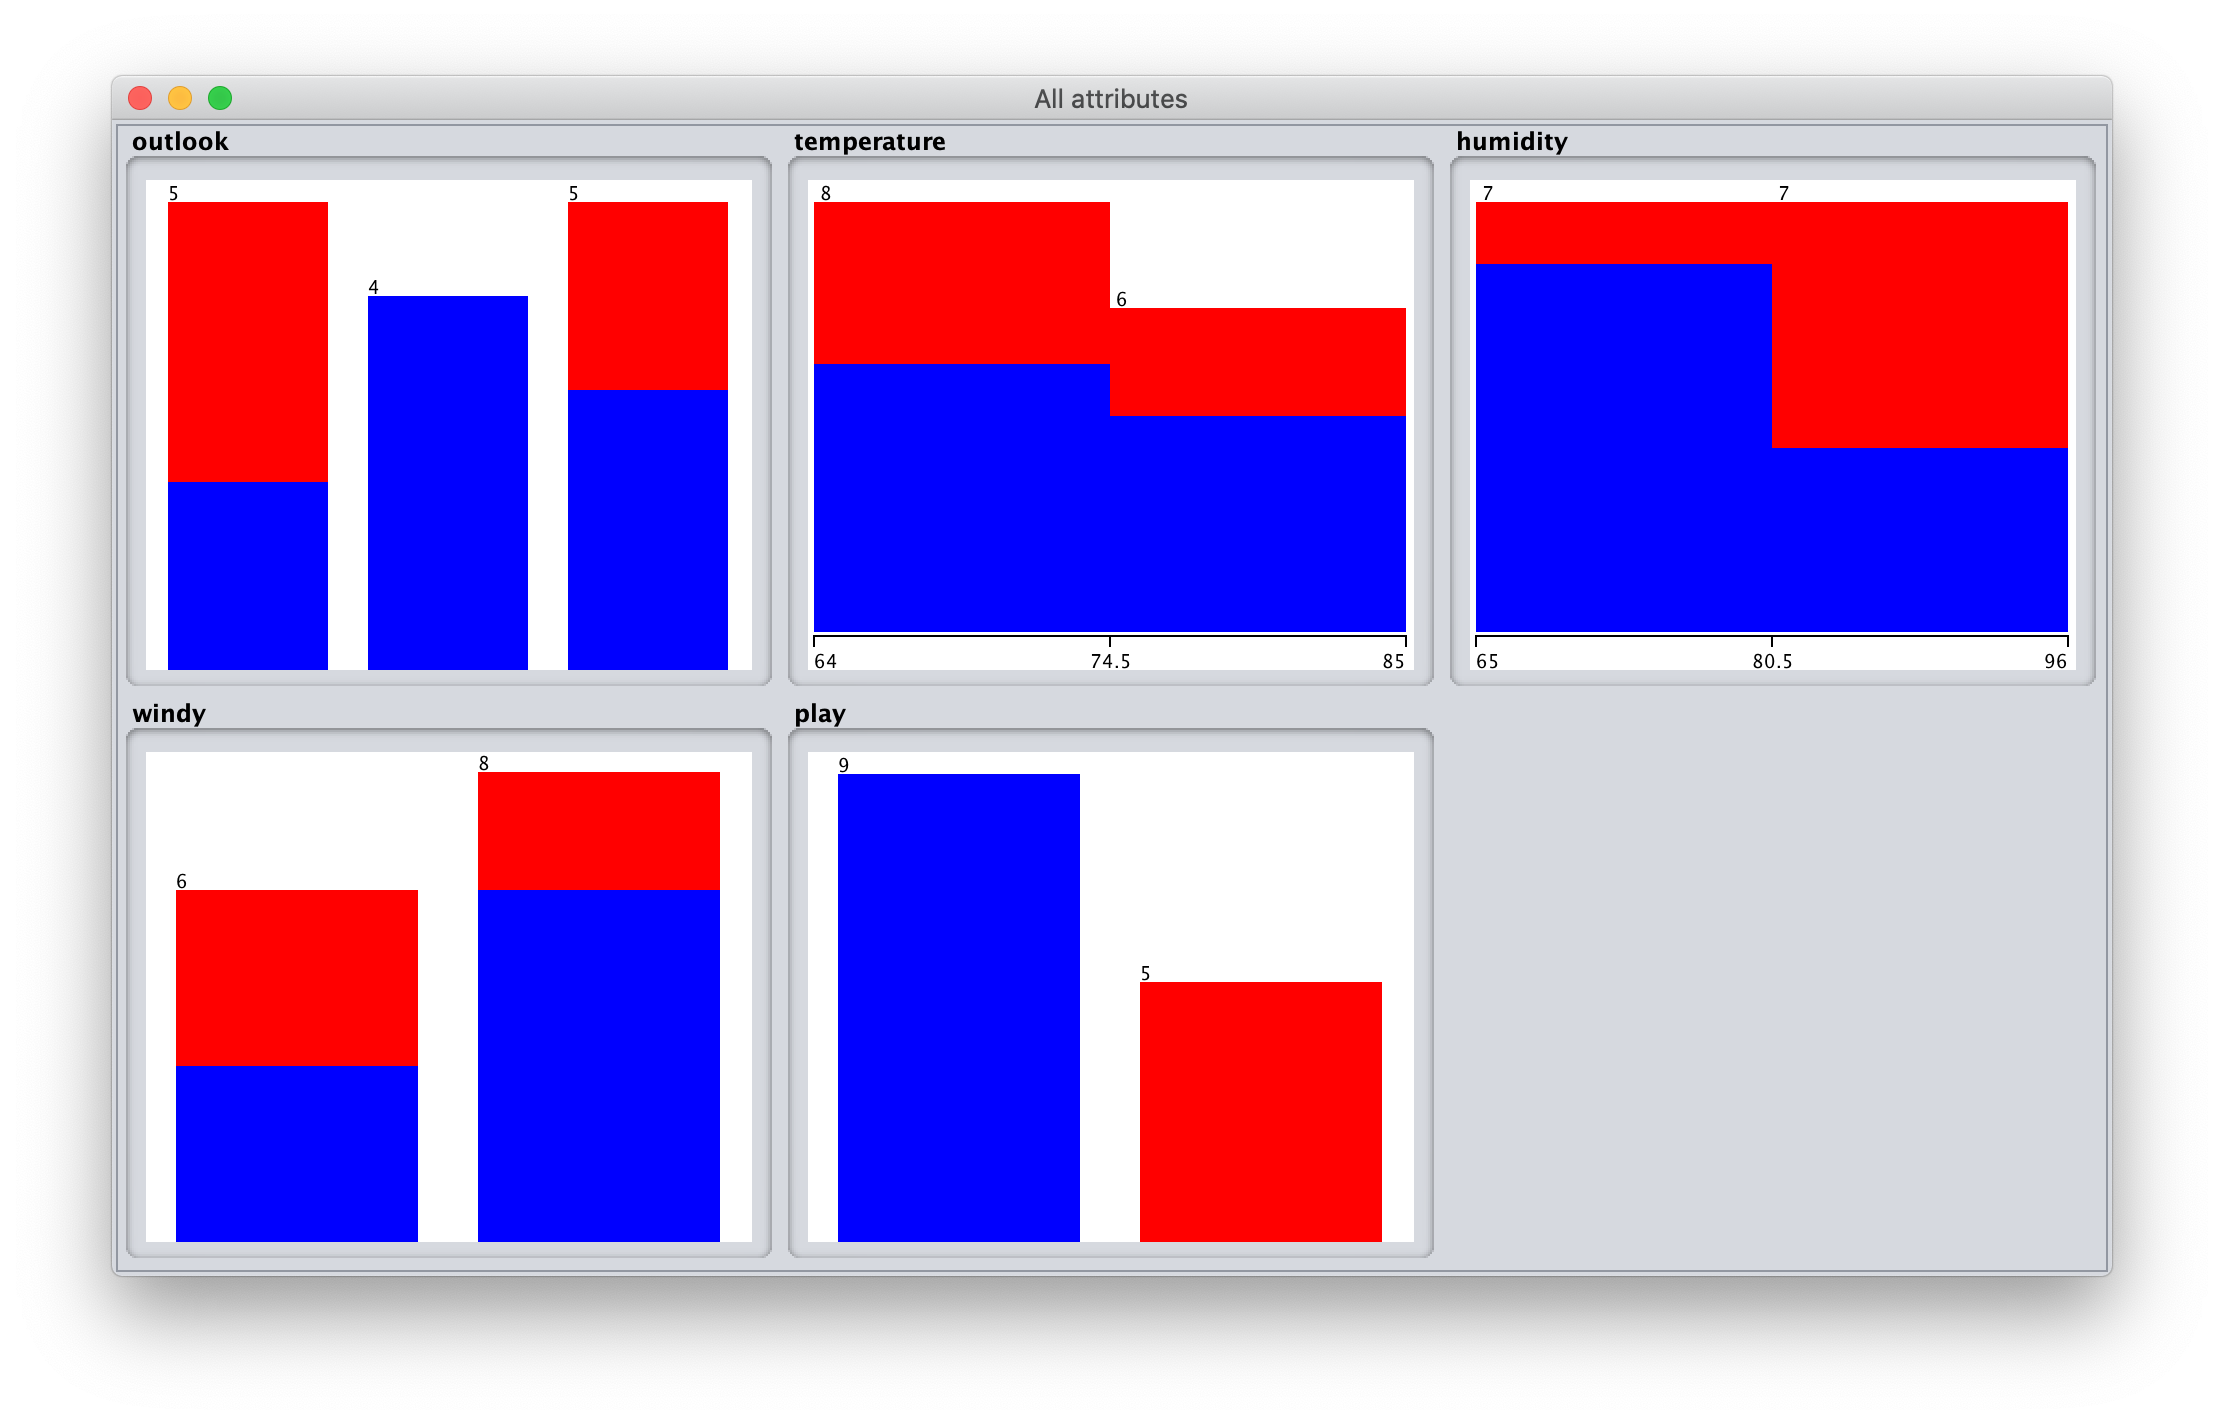
\includegraphics[scale = 0.45]{images/weather_diagram.png}
            \caption{Đồ thị biểu diễn các thuộc tính của tập dữ liệu của tập weather}
        \end{center}
    \end{figure}

    \item Thuật ngữ sử dụng cho các đồ thị ở tab Visualize là đồ thị phân tán (scatter plot)
    \begin{figure}[H]
        \begin{center}
            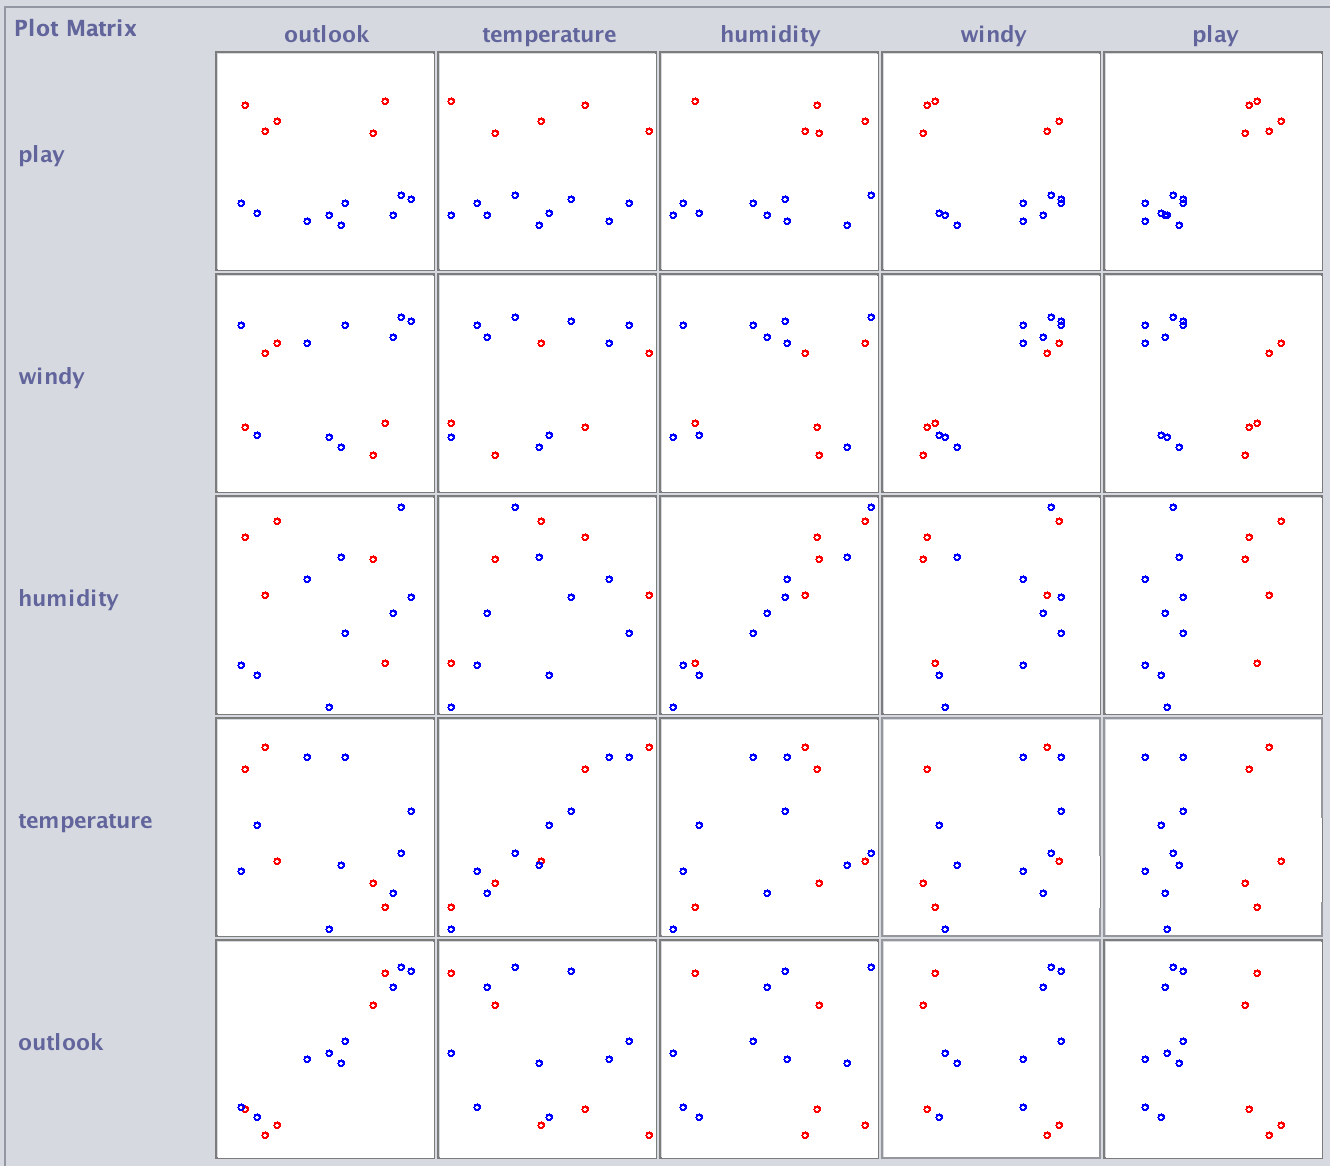
\includegraphics[scale = 0.5]{images/weatherScatterPlot.png}
            \caption{Đồ thị phân tán của các thuộc tính trong tập dữ liệu Weather}
        \end{center}
    \end{figure}

    \item Dựa vào các đồ thị quan sát được, theo phán đoán của nhóm, cặp dữ liệu \textit{outlook - play} có vẻ như tương quan với nhau
\end{itemize}

\subsection{Khám phá tập dữ liệu Tín dụng Đức}

\begin{itemize}
    \item Nội dung chú thích ở đầu tập tin mô tả về tập dữ liệu tín dụng Đức. Phần mô tả bao gồm tiêu đề, thông tin về nguồn gốc của tập tin, số lượng mẫu, số lượng thuộc tính và loại dữ liệu của các thuộc tính và mô tả chi tiết về thuộc tính. Ngoài ra, phần chú thích còn cho biết thêm về ma trận chi phí và ánh xạ ý nghĩa của giá trị của thuộc tính với ký hiệu hiển thị trên giao diện. Tập thuộc tính có 1000 mẫu với 21 thuộc tính. Dưới đây là thông tin về 5/21 thuộc tính có trong tập dữ liệu
    \begin{itemize}
        \item duration (thuộc tính rời rạc): thời hạn vay tín dụng (tính theo tháng)

        \item credit\_history (thuộc tính rời rạc): lịch sử tín dụng, bao gồm 5 trạng thái
        \begin{itemize}
            \item Không có tín dụng nào được thực hiện hoặc các khoản tín dụng được trả một cách hợp lệ
            \item Tất cả các tín dụng ở ngân hàng này đều được trả một cách hợp lệ 
            \item Các khoản tín dụng đã được hoàn trả hợp lệ cho đến nay
            \item Trong quá khứ đã từng hoàn trả tín dụng muộn 
            \item Tài khoản tín dụng quan trọng hoặc đã tồn tại tài khoản tín dụng ở ngân hàng khác
        \end{itemize}

        \item purpose (thuộc tính rời rạc): mục đích của việc vay tín dụng
        \begin{itemize}
            \item Mua xe mới
            \item Mua xe đã qua sử dụng
            \item Mua đồ nội thất
            \item Mua radio/TV
            \item Mua thiết bị gia dụng
            \item Sửa chữa
            \item Chi trả cho giáo dục
            \item Đi nghỉ dưỡng
            \item Chi trả chi phí đào tạo lại
            \item Đầu tư kinh doanh
            \item Khác 
        \end{itemize}

        \item saving\_status (thuộc tính liên tục): tài khoản tiết kiệm, được chia ra các mức
        \begin{itemize}
            \item Nhỏ hơn 100 Mark Đức\footnote{Đơn vị tiền tệ của Đức}
            \item Nằm trong khoảng 100 và 500 Mark Đức
            \item Nằm trong khoảng 500 và 1000 Mark Đức
            \item Lớn hơn 1000 Mark Đức
        \end{itemize}

        \item persional\_status (thuộc tính rời rạc): giới tính và trạng thái hiện tại của một người
        \begin{itemize}
            \item Nam, ly thân
            \item Nữ, ly thân hoặc đã có gia đình
            \item Nam, độc thân
            \item Nữ độc thân
            \item Nam đã có gia đình hoặc goá vợ
        \end{itemize}
    \end{itemize}

    \item Tên thuộc tính lớp: class (bao gồm 2 giá trị là good và bad). Cân bằng lệch về phía good

    \item Phương pháp chọn lọc thuộc tính của Weka trong tab Select attributes
    \begin{itemize}
        \item \textbf{GainRatioAttributeEval}: Độ đo này được sử dụng trong thuật toán C4.5 do Quinlan đưa ra năm 1993. Ý tưởng của thuật toán là xét tất cả các phép thử có thể phân chia tập dữ liệu đã cho và chọn ra một phép thử cho GainRatio tốt nhất. GainRatio cũng là một độ đo sự hiệu quả của một thuộc tính trong thuật toán triển khai cây quyết định 
        $$GainRatio(S, A) = \frac{Gain(S, A)}{SplitInformation(S, A)}$$ $$SplitInformation(S, A) = -  \sum_{i=1}^{c} (\frac{|S_i|}{|S|} \log_2 \frac{|S_i|}{|S|})$$
        \begin{itemize}
            \item $S_i$ là tập con của $S$ với $A$ có giá trị $v_i$
        \end{itemize}

        \item \textbf{InfoGainAttributeEval}: Đo mức hiệu quả của một thuộc tính trong bài toán phân lớp dữ liệu 
        $$Gain(S, A) = Entropy(S) - \sum_{v \in Value(A)} [\frac{S_v}{S}Entropy(S_v)]$$ $$Entropy(S) = \sum_{i = 1}^{c} (-p_i \log_2 p_i)$$
        \begin{itemize}
            \item $p_i$ là tỉ lệ của các mẫu thuộc lớp $i$ trong tập $S$
            \item $Value(A)$ là tập tất cả các giá trị có thể có đối với thuộc tính $A$
            \item $S_v$ là tập con của $S$ mà $A$ có giá trị là $v$
        \end{itemize}

        \item Ngoài ra còn rất nhiều options để lọc thuộc tính tuỳ theo ý đồ của người sử dụng.
    \end{itemize}

    \item Theo như mô tả trên thì việc chọn \textbf{GainRatioAttributeEval} hay \textbf{InfoGainAttributeEval} đều cho biết về các thuộc tính có tương quan cao nhất đối với thuộc tính lớp. Trong báo cáo, người viết chọn \textbf{InfoGainAttributeEval} để chọn các thuộc tính này.
    \begin{itemize}
        \item Bước 1: Chọn vào tab Select attributes. Tại mục Attribute Evaluator, chọn \textbf{InfoGain\\AttributeEval}. Tại mục Search Method, chọn \textbf{Ranker}
        \begin{figure}[H]
            \begin{center}
                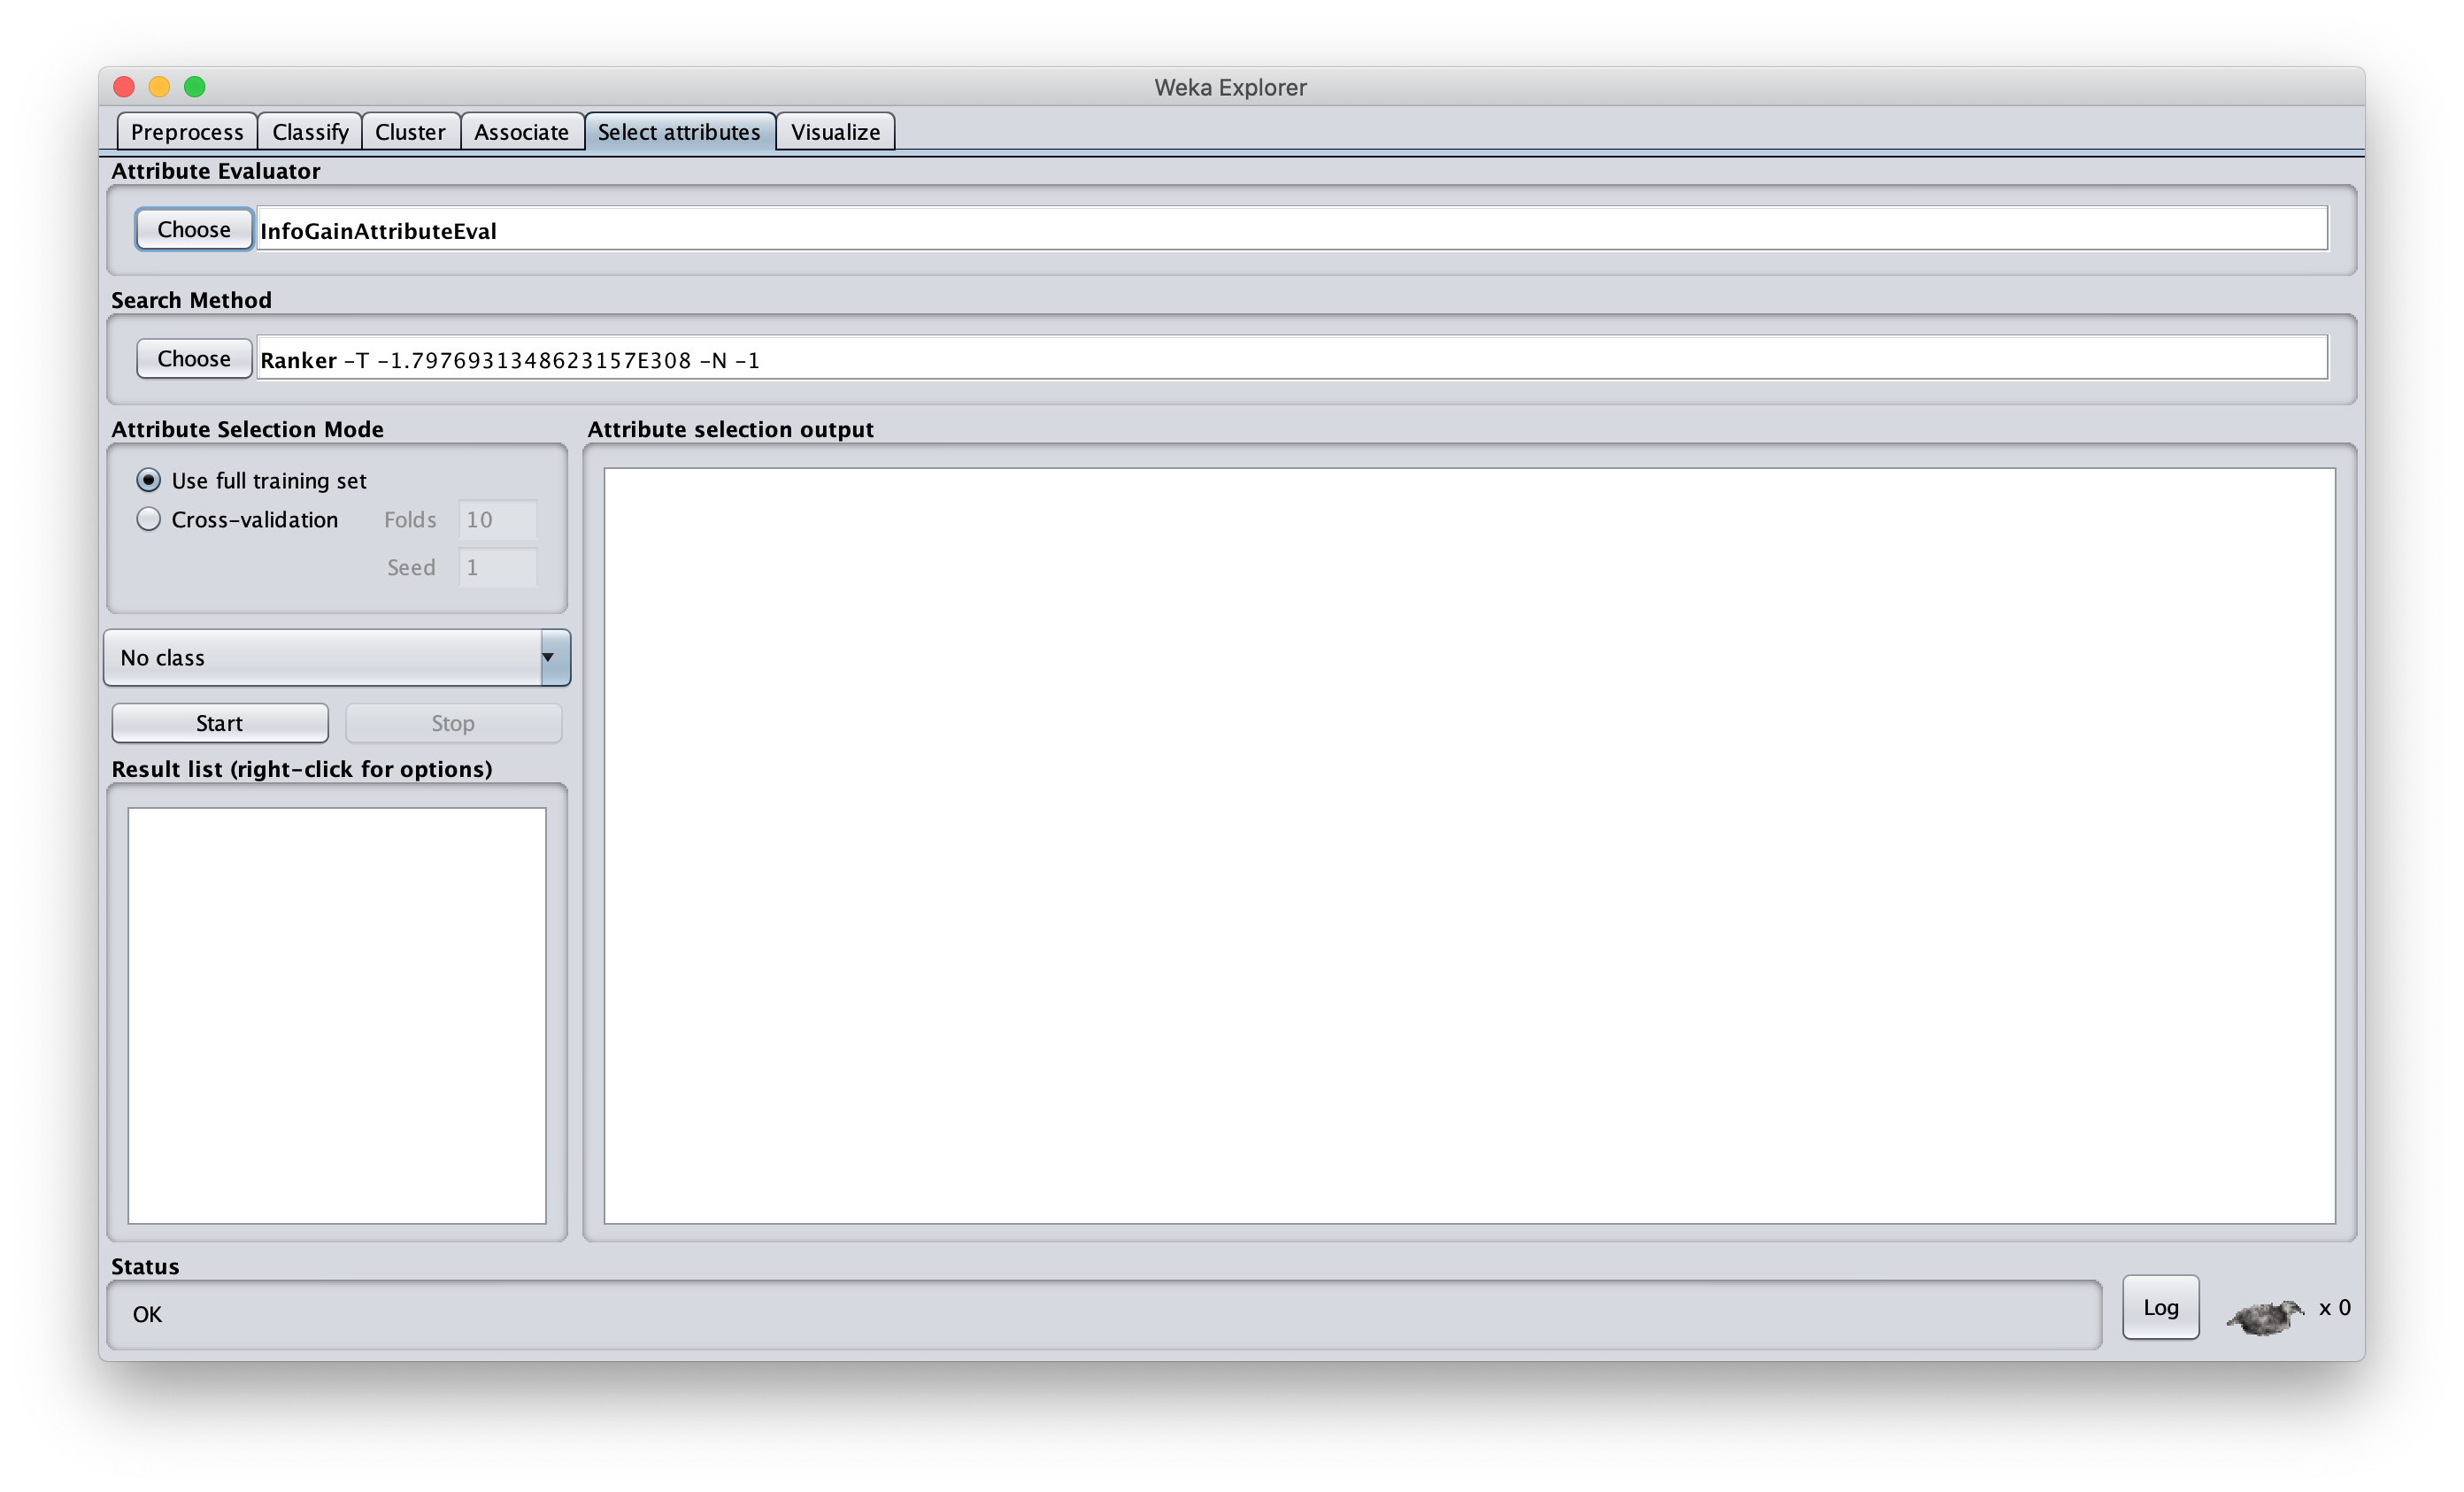
\includegraphics[scale = 0.35]{images/selectAttributeCreditG.png}
                \caption{Chọn Attribute Evaluator và Search Method}
            \end{center}
        \end{figure}
        \item Bước 2: Nhấn nút Start
        \item Bước 3: Đọc kết quả
        \begin{figure}[H]
            \begin{center}
                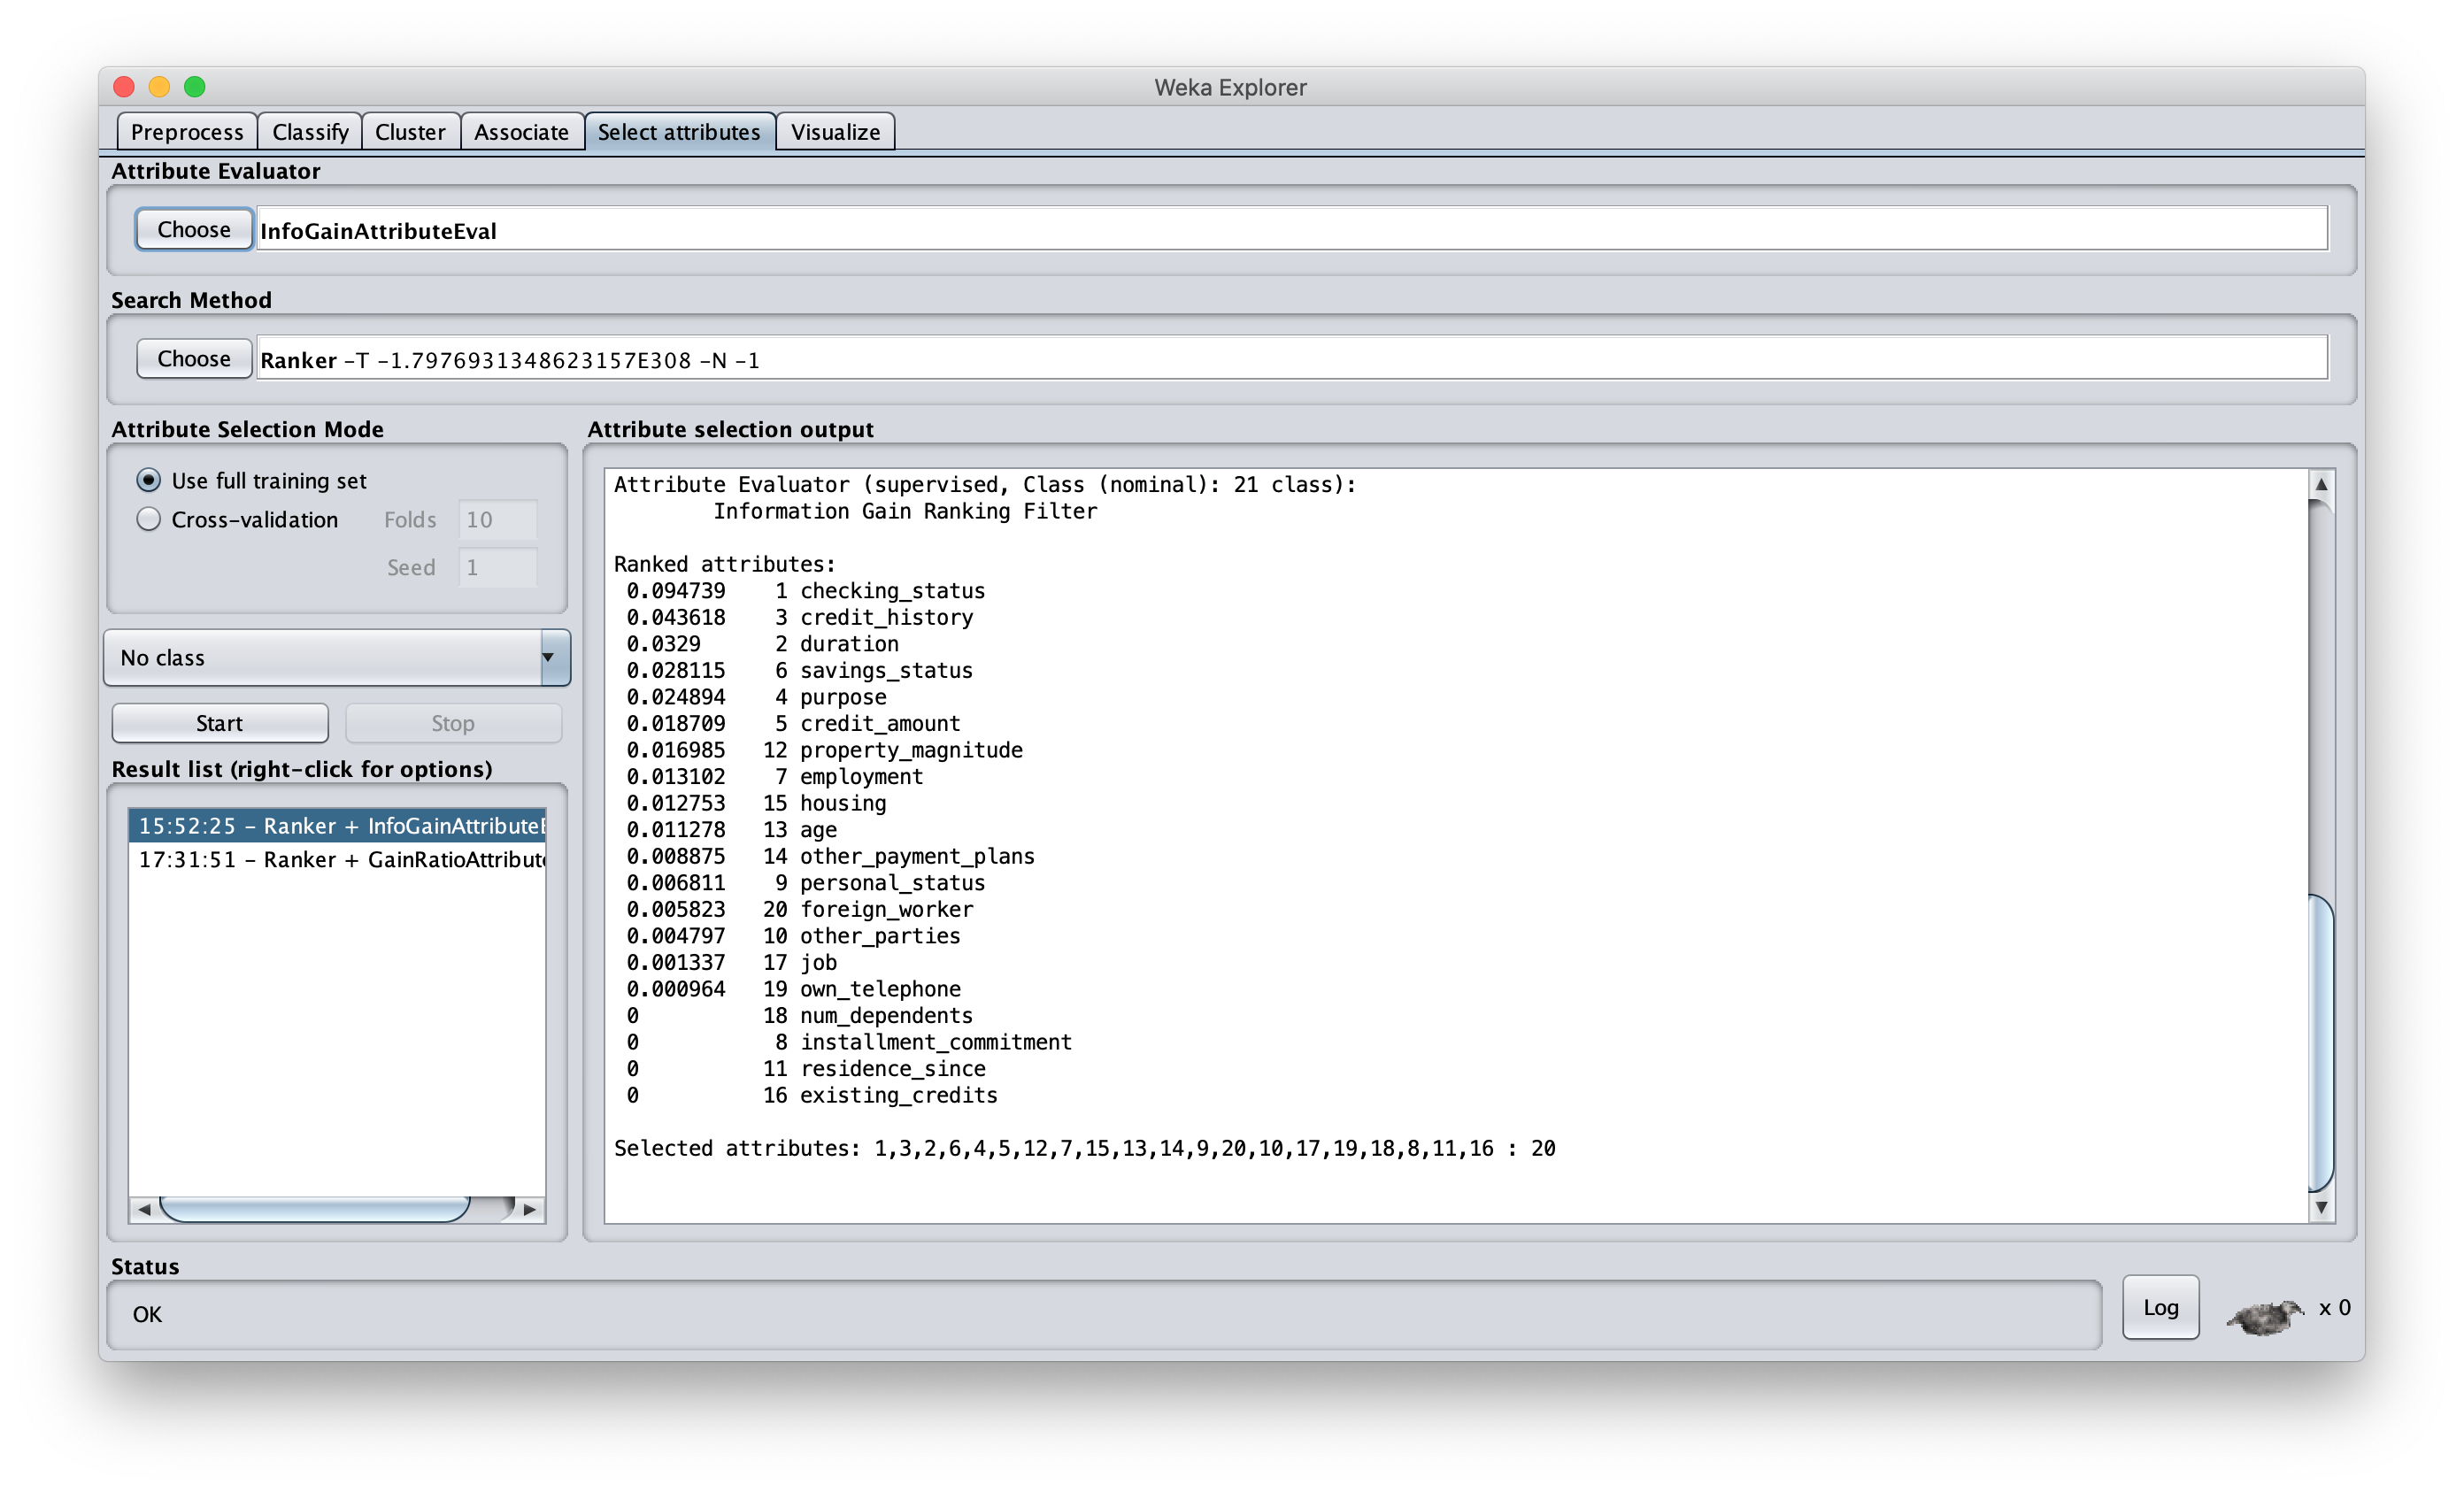
\includegraphics[scale = 0.35]{images/creditG_result.png}
                \caption{Danh sách các thuộc tính có tương quan cao nhất đối với thuộc tính lớp}
            \end{center}
        \end{figure}
    \end{itemize}

    \item Từ hình trên, ta có thể thấy 5 thuộc tính có tương quan cao nhất với thuôc tính lớp là \textbf{checking\_status, credit\_history, duration, saving\_status, purpose}
\end{itemize}

\clearpage

\section{Yêu cầu 3: Cài đặt tiền xử lý dữ liệu}
\begin{itemize}
    \item Trong thư mục \textbf{Result}, nhóm đồ án đã có đính kèm tất cả các dữ liệu đầu ra của chương trình kèm theo mô tả trong file \textbf{README.md}
    \item Đường dẫn: \url{https://github.com/baolongnguyenmac/DataMining-Lab1/tree/main/Result}
\end{itemize}

\begin{enumerate}
    \item Liệt kê các cột bị thiếu dữ liệu
    \begin{itemize}
        \item Cú pháp: python main.py -type listmissingdata -filein <fileName>
        \item Kết quả: Chương trình in ra dánh sách các cột bị thiếu dữ liệu
        \begin{figure}[H]
            \begin{center}
                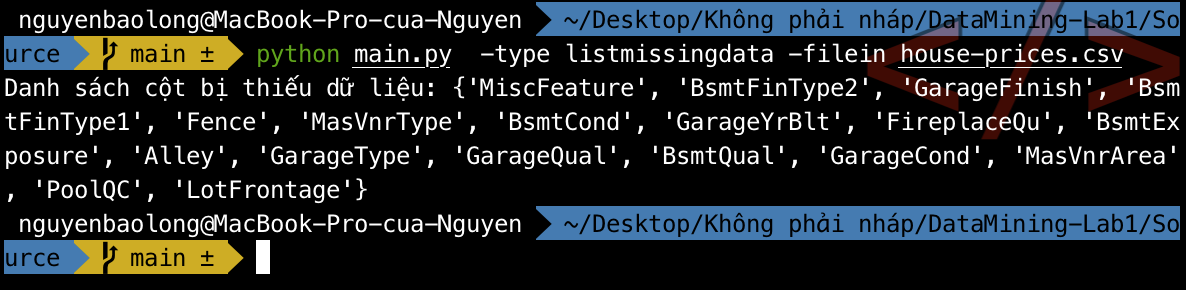
\includegraphics[scale = 0.75]{images/listmissingdata.png}
                \caption{Kết quả sau khi liệt kê các thuộc tính bị mất dữ liệu}
            \end{center}
        \end{figure}
    \end{itemize}

    \item Đếm số dòng bị thiếu dữ liệu
    \begin{itemize}
        \item Cú pháp: python main.py -type countmissingdata -filein <fileName>
        \item Kết quả: Chương trình in ra số dòng bị thiếu dữ liệu
        \begin{figure}[H]
            \begin{center}
                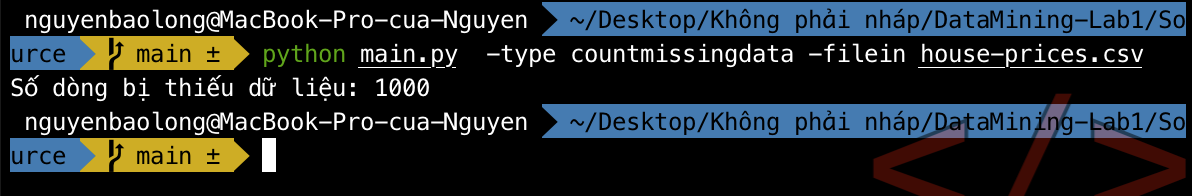
\includegraphics[scale = 0.75]{images/missingdata.png}
                \caption{Kết quả sau khi đếm số dòng bị thiếu dữ liệu}
            \end{center}
        \end{figure}
    \end{itemize}

    \item Điền giá trị thiếu
    \begin{itemize}
        \item Cú pháp
        \begin{itemize}
            \item python main.py -type fillmissingdata -method mean -filein <fileName> -fileout <fileName>
            \item python main.py -type fillmissingdata -method median -filein <fileName> -fileout <fileName>
        \end{itemize}

        \item Kết quả: Dữ liệu sau khi xử lý được lưu trong file kết quả
    \end{itemize}

    \item Xoá các dòng bị thiếu dữ liệu
    \begin{itemize}
        \item Cú pháp: python main.py -type eraserow -rate <rate> -filein <fileName> -fileout <fileName>
        \item Kết quả: Dữ liệu sau khi xử lý được lưu trong file kết quả
    \end{itemize}

    \item Xoá các cột bị thiếu dữ liệu
    \begin{itemize}
        \item Cú pháp: python main.py -type erasecolumn -rate <rate> -filein <fileName> -fileout <fileName>
        \item Kết quả: Dữ liệu sau khi xử lý được lưu trong file kết quả
    \end{itemize}

    \item Xoá các mẫu bị trùng lặp
    \begin{itemize}
        \item Cú pháp: python main.py -type eraseduplicaterow -filein <fileName> -fileout <fileName>
        \item Kết quả: Dữ liệu sau khi xử lý được lưu trong file kết quả
    \end{itemize}

    \item Chuẩn hoá một thuộc tính
    \begin{itemize}
        \item Cú pháp
        \begin{itemize}
            \item python main.py -type standardize -method minmax -attribute <attribute> -filein <fileName> -fileout <fileName>
            \item python main.py -type standardize -method zscore -attribute <attribute> -filein <fileName> -fileout <fileName>
        \end{itemize}

        \item Kết quả: Dữ liệu sau khi chuẩn hoá được lưu trong file kết quả
    \end{itemize}

    \item Tính giá trị biểu thức
    \begin{itemize}
        \item Cú pháp: python main.py -type expression
        \item Kết quả: Chương trình cho người dùng nhập biểu thức trên màn hình Console. Kết quả của biểu thức được lưu thành 1 thuộc tính mới (có tên trùng với biểu thức nhập vào) trong file kết quả
    \end{itemize}

\end{enumerate}

\end{document}